\subsection{Iteraciones}
El proyecto se dividió en 11 iteraciones, cada una con una duración entre una y tres semanas para su realización y, con un número determinado de historias de usuario. Cada una de estas historias se dividieron en tareas llamadas “Tareas de Ingeniería”, asimismo, para cada una de ellas se definieron “Casos de pruebas de aceptación”, los cuales se realizaron en la culminación de las mismas.

Para el desarrollo de cada iteración, se hizo uso de GitHub (sistema de control de versiones) para facilitar la integración del código de los dos desarrolladores.

Cabe señalar que, al finalizar cada iteración, los desarrolladores se reunían con el Manager del proyecto para hacer la respectiva entrega y revisar avances del proyecto. Es importante resaltar que, aunque las entregas fueron planeadas para su realización, en algunos casos por cambios en las mismas, no se cumplió con los entregables acordados, o en otros casos se había avanzado más de lo acordado. 

A continuación, se menciona la iteración 1 con sus respectivas tareas y casos de pruebas aceptación.

\textbf{Iteración 1: }\ \\
La iteración 1, comprende a las siguientes historias de usuario:
\begin{itemize}
    \item Historia de usuario Nº 1: Registrar estudiante
    \item Historia de usuario Nº 4: Iniciar sesión del usuario
    \item Historia de usuario Nº 31: Cerrar sesión del usuario
\end{itemize}

Las tareas realizadas en esta iteración fueron:

\begin{figure}[H]
\begin{tabular}{|p{4cm}|p{4cm}|p{4cm}|p{4cm}|}
\hline
\multicolumn{4}{|>{\columncolor[rgb]{0.9,0.9,0.9}}r|}{ \textbf{Tarea de Ingeniería}}\\
\hline
\textbf{Número de Tarea: } &\multicolumn{3}{|p{12cm}|}{\textbf{Historia de Usuario} (N$^{\circ}$ y Nombre):}\\
N$^{\circ}$1& \multicolumn{3}{|p{12cm}|}{1 – Registrar Estudiante}\\
\hline
\multicolumn{4}{|p{16cm}|}{ \textbf{Nombre Tarea: }Desarrollo del módulo de registro estudiante}\\
\hline
\multicolumn{2}{|p{8cm}|}{\textbf{Tipo de Tarea:} Desarrollo }&\multicolumn{2}{|p{8cm}|}{\textbf{Puntos Estimados:} 3 }\\
\hline
\multicolumn{2}{|p{8cm}|}{\textbf{Fecha de Inicio:} 24/04/2018 }&\multicolumn{2}{|p{8cm}|}{\textbf{Fecha de culminación:} 28/04/2018 }\\
\hline
\multicolumn{4}{|p{16cm}|}{ \textbf{Programador Responsable: }}\\
\multicolumn{4}{|p{16cm}|}{ Natalia Rubiano Silva}\\
\hline
\multicolumn{4}{|p{16cm}|}{\textbf{Descripción: }Desarrollar el módulo de registro de estudiantes, mediante el cual un usuario digitando sus datos (nombre, correo y contraseña) correctamente se guardarán en una base de datos y así podrá ingresar al sistema.}\\
\hline
\end{tabular}
    \caption{Tarea Nº1 - Iteración 1}
    \centering \scriptsize \textbf{Fuente:} Elaboración propia
\end{figure}

\begin{figure}[H]
\begin{tabular}{|p{4cm}|p{4cm}|p{4cm}|p{4cm}|}
\hline
\multicolumn{4}{|>{\columncolor[rgb]{0.9,0.9,0.9}}r|}{ \textbf{Tarea de Ingeniería}}\\
\hline
\textbf{Número de Tarea: } &\multicolumn{3}{|p{12cm}|}{\textbf{Historia de Usuario} (N$^{\circ}$ y Nombre):}\\
N$^{\circ}$2& \multicolumn{3}{|p{12cm}|}{4 – Iniciar sesión del usuario}\\
\hline
\multicolumn{4}{|p{16cm}|}{ \textbf{Nombre Tarea: }Desarrollo del módulo de iniciar sesión}\\
\hline
\multicolumn{2}{|p{8cm}|}{\textbf{Tipo de Tarea:} Desarrollo }&\multicolumn{2}{|p{8cm}|}{\textbf{Puntos Estimados:} 3 }\\
\hline
\multicolumn{2}{|p{8cm}|}{\textbf{Fecha de Inicio:} 30/04/2018 }&\multicolumn{2}{|p{8cm}|}{\textbf{Fecha de culminación:} 04/05/2018 }\\
\hline
\multicolumn{4}{|p{16cm}|}{ \textbf{Programador Responsable: }}\\
\multicolumn{4}{|p{16cm}|}{ Natalia Rubiano Silva}\\
\hline
\multicolumn{4}{|p{16cm}|}{\textbf{Descripción: }Desarrollar el módulo de iniciar sesión, donde el usuario se autentica con correo y contraseña.}\\
\hline
\end{tabular}
    \caption{Tarea Nº2 - Iteración 1}
    \centering \scriptsize \textbf{Fuente:} Elaboración propia
\end{figure}

Algunos casos de Pruebas de aceptación realizados para esta iteración fueron: 

\begin{figure}[H]
\begin{tabular}{|p{4cm}|p{4cm}|p{4cm}|p{4cm}|}
\hline
\multicolumn{4}{|>{\columncolor[rgb]{0.9,0.9,0.9}}r|}{ \textbf{Caso de Prueba de Aceptación}}\\
\hline
\textbf{Número de caso de} &\multicolumn{3}{|p{12cm}|}{\textbf{Historia de Usuario} (N$^{\circ}$ y Nombre):}\\
\textbf{Prueba: }N$^{\circ}$1 & \multicolumn{3}{|p{12cm}|}{1- Registrar Estudiante}\\
\hline
\multicolumn{4}{|p{16cm}|}{ \textbf{Nombre: }Prueba del módulo de registro de estudiantes}\\
\hline
\multicolumn{4}{|p{16cm}|}{\textbf{Descripción: }Se probará que el sistema permita el registro de estudiantes.}\\
\hline
\multicolumn{4}{|p{16cm}|}{\textbf{Condiciones de Ejecución: }}\\
\multicolumn{4}{|p{16cm}|}{
    - El estudiante no puede estar registrado en la aplicación.}\\
\hline
\multicolumn{4}{|p{16cm}|}{\textbf{Entrada / Pasos de ejecución: }}\\
\multicolumn{4}{|p{16cm}|}{- El estudiante accede al módulo de registro.}\\
\multicolumn{4}{|p{16cm}|}{- El estudiante digita su nombre.}\\
\multicolumn{4}{|p{16cm}|}{- El estudiante digita sus apellidos}\\
\multicolumn{4}{|p{16cm}|}{- El estudiante digita su correo}\\
\multicolumn{4}{|p{16cm}|}{- El estudiante digita su su contraseña}\\
\multicolumn{4}{|p{16cm}|}{- El estudiante da clic sobre el botón registrar.}\\
\hline
\multicolumn{4}{|p{16cm}|}{\textbf{Resultado Esperado: }}\\
\multicolumn{4}{|p{16cm}|}{El estudiante quedará registrado en el sistema y accederá a él.}\\
\hline
\multicolumn{4}{|p{16cm}|}{\textbf{Evaluación de la Prueba:  }}\\
\multicolumn{4}{|p{16cm}|}{Prueba satisfactoria.}\\
\hline
\end{tabular}
    \caption{Caso de Prueba de Aceptación Nº1 - Iteración 1}
    \centering \scriptsize \textbf{Fuente:} Elaboración propia
\end{figure}

\begin{figure}[H]
\begin{tabular}{|p{4cm}|p{4cm}|p{4cm}|p{4cm}|}
\hline
\multicolumn{4}{|>{\columncolor[rgb]{0.9,0.9,0.9}}r|}{ \textbf{Caso de Prueba de Aceptación}}\\
\hline
\textbf{Número de caso de} &\multicolumn{3}{|p{12cm}|}{\textbf{Historia de Usuario} (N$^{\circ}$ y Nombre):}\\
\textbf{Prueba: }N$^{\circ}$2 & \multicolumn{3}{|p{12cm}|}{1 - Registrar Estudiante}\\
\hline
\multicolumn{4}{|p{16cm}|}{ \textbf{Nombre: }Prueba de casillas vacías del módulo de registro de estudiantes}\\
\hline
\multicolumn{4}{|p{16cm}|}{\textbf{Descripción: }Se probará que un estudiante no pueda dejar casillas vacías cuando intente registrarse al sistema.}\\
\hline
\multicolumn{4}{|p{16cm}|}{\textbf{Condiciones de Ejecución: }}\\
\multicolumn{4}{|p{16cm}|}{- El estudiante no puede estar registrado en la aplicación.}\\
\hline
\multicolumn{4}{|p{16cm}|}{\textbf{Entrada / Pasos de ejecución: }}\\
\multicolumn{4}{|p{16cm}|}{- El estudiante accede al módulo de registro.}\\
\multicolumn{4}{|p{16cm}|}{- El estudiante digita su nombre.}\\
\multicolumn{4}{|p{16cm}|}{- El estudiante digita sus apellidos}\\
\multicolumn{4}{|p{16cm}|}{- El estudiante deja la casilla de correo vacía.}\\
\multicolumn{4}{|p{16cm}|}{- El estudiante digita su contraseña.}\\
\multicolumn{4}{|p{16cm}|}{- El estudiante da clic sobre el botón registrar.}\\
\hline
\multicolumn{4}{|p{16cm}|}{\textbf{Resultado Esperado: }}\\
\multicolumn{4}{|p{16cm}|}{Mensaje de “Completar el campo”.}\\
\hline
\multicolumn{4}{|p{16cm}|}{\textbf{Evaluación de la Prueba:  }}\\
\multicolumn{4}{|p{16cm}|}{Prueba satisfactoria.}\\
\hline
\end{tabular}
    \caption{Caso de Prueba de Aceptación Nº2 - Iteración 1}
    \centering \scriptsize \textbf{Fuente:} Elaboración propia
\end{figure}

Ahora bien, el trabajo del desarrollo de las historias de usuarios y el de las pruebas de aceptación fue ejecutado por separado por un programador diferente, es decir, quien desarrolló una historia de usuario, fue diferente a quien desarrolló las pruebas de aceptación del mismo.

Para mayor detalle acerca de las iteraciones realizadas ver \textbf{(Carpeta Anexos, documento: Iteraciones)}

\subsubsection{Descripción de la aplicación}
Finalizadas las iteraciones se obtiene como producto final una aplicación hipermedia con características adaptativas para el aprendizaje física (denominado Fisimatica). A continuación, se muestran las interfaces principales del usuario: 

\begin{figure}[H]
    \centering
    \begin{subfigure}[b]{0.4\textwidth}
        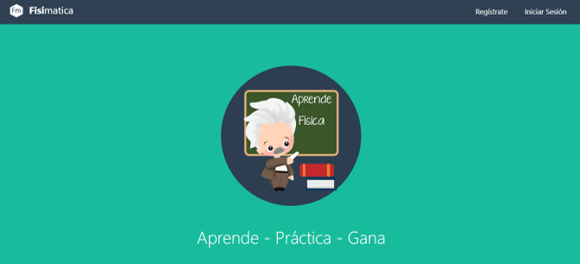
\includegraphics[width=\textwidth]{Capitulo_4/2_XP/imagenes/inicio.png}
        \caption{Página inicial de la aplicación}
        \label{fig:gull}
    \end{subfigure}
    ~ %add desired spacing between images, e. g. ~, \quad, \qquad, \hfill etc. 
      %(or a blank line to force the subfigure onto a new line)
    \begin{subfigure}[b]{0.4\textwidth}
        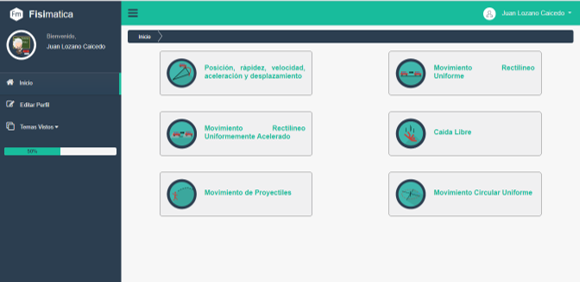
\includegraphics[width=\textwidth]{Capitulo_4/2_XP/imagenes/navL.png}
        \caption{Navegación libre de la aplicación}
        \label{fig:tiger}
    \end{subfigure}
    \par \bigskip
    \begin{subfigure}[b]{0.4\textwidth}
        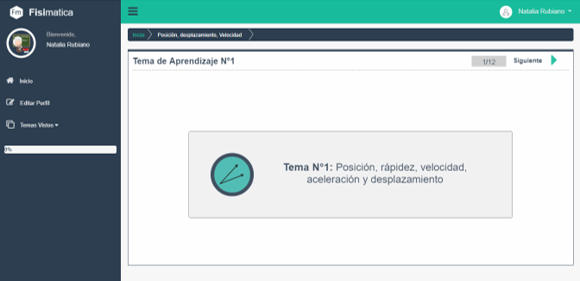
\includegraphics[width=\textwidth]{Capitulo_4/2_XP/imagenes/navG.png}
        \caption{Navegación guiada de la aplicación}
        \label{fig:tiger}
    \end{subfigure}
    \caption{Interfaces principales de la aplicación}\label{fig:interfaz}
\end{figure}



